\documentclass[crop,tikz]{standalone}

\usepackage{pgfplots}
\pgfplotsset{compat=1.17}

\definecolor{col2}{HTML}{ff595e}
\definecolor{col3}{HTML}{8ac926}
\definecolor{col4}{HTML}{1982c4}
\definecolor{col5}{HTML}{6a4c93}
\definecolor{col6}{HTML}{577590}

\begin{document}

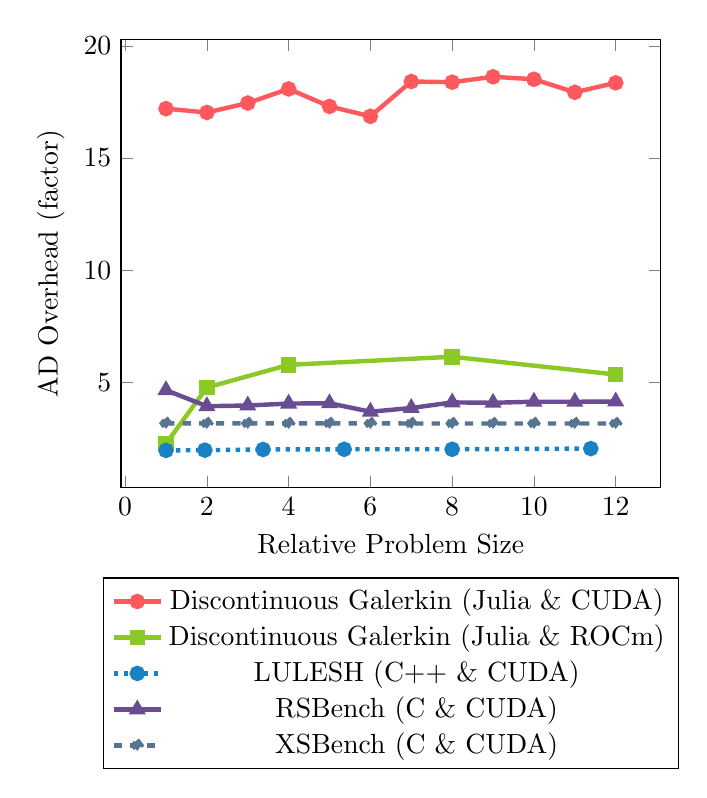
\begin{tikzpicture}
   \begin{axis}[%ymode=log,
                xlabel = {Relative Problem Size},
                ylabel = {AD Overhead (factor)},
                legend style={
                    %area legend,
                    at={(0.5,-0.2)},
                    anchor=north,
                    legend columns=1}
                    ]
      % DG (CUDA)
      \addplot[ultra thick, col2, mark=*] coordinates {(1,17.20) (2,17.03) (3,17.45) (4,18.08) (5,17.30) (6, 16.86) (7, 18.41) (8, 18.38) (9, 18.62) (10, 18.51) (11, 17.93) (12, 18.35)};
      % DG (ROCm)
      \addplot[ultra thick, col3, mark=square*] coordinates {(1,2.28) (2,4.78) (4,5.79) (8,6.15) (12,5.36)};
      % LULESH
      \addplot[ultra thick, col4, dotted, every mark/.append style={solid, fill=gray}, mark=otimes*] coordinates {(1,1.98) (1.95, 1.99) (3.375, 2.02) (5.359375, 2.03) (8, 2.03) (11.390625, 2.06)};
      % RSBench
      \addplot[ultra thick, col5, mark=triangle*] coordinates {(1,4.661582459) (2, 3.948345035) (3, 3.979550102) (4, 4.065775681) (5, 4.079569439) (6, 3.702369516) (7, 3.867231233) (8, 4.117181417) (9, 4.101083883) (10, 4.147683398) (11, 4.145880059) (12, 4.157394113)};
      % XSBench
      \addplot[ultra thick, col6, dashed, mark=diamond*] coordinates {(1,3.183) (2, 3.182) (3, 3.181) (4, 3.180) (5, 3.181) (6, 3.180) (7, 3.179) (8, 3.178) (9, 3.178) (10, 3.178) (11, 3.178) (12, 3.178)};
      \legend{{Discontinuous Galerkin (Julia \& CUDA)},
              {Discontinuous Galerkin (Julia \& ROCm)},
              {LULESH (C++ \& CUDA)},
              {RSBench (C \& CUDA)},
              {XSBench (C \& CUDA)}}
   \end{axis}
\end{tikzpicture}

\end{document}